\documentclass[aspectratio=169,10pt]{beamer}

% ─── Packages ────────────────────────────────────────────────────────────────
\usepackage{amsmath,amssymb,bm}
\usepackage{graphicx}
\usepackage{tikz}
\usetikzlibrary{arrows.meta,shapes.geometric,positioning,fit,calc,shadows}
\usepackage{booktabs}
\usepackage{colortbl}
\usepackage{xcolor}
\usepackage{multirow}
\usepackage{array}
\usepackage{mathtools}

% ─── Colour Palette ──────────────────────────────────────────────────────────
\definecolor{oceanblue}{RGB}{10,46,90}
\definecolor{midblue}{RGB}{21,101,192}
\definecolor{cyancol}{RGB}{0,172,193}
\definecolor{surfaceblue}{RGB}{227,242,253}
\definecolor{warnred}{RGB}{183,28,28}
\definecolor{okgreen}{RGB}{27,94,32}
\definecolor{lightgray}{RGB}{248,249,250}
\definecolor{tablegray}{RGB}{236,239,241}
\definecolor{dlnncolor}{RGB}{13,71,161}

% ─── Theme Configuration ─────────────────────────────────────────────────────
\usetheme{Madrid}
\usecolortheme{default}

\title[AUV Trajectory Tracking]{Replication and Evaluation: AUV Control Strategies}
\subtitle{Double-Loop PID-Type Neural Network Sliding Mode Control}
\author{Student Name}
\institute{Department of Marine Engineering}
\date{\today}

\begin{document}

% ══════════════════════════════════════════════════════════════════════════════
% SLIDE 1 – Title
% ══════════════════════════════════════════════════════════════════════════════
{
\setbeamertemplate{footline}{}
\begin{frame}[plain]
  \begin{tikzpicture}[remember picture, overlay]
    % Ocean gradient background
    \fill[oceanblue] (current page.south west) rectangle (current page.north east);
    % Decorative wave strip
    \fill[midblue!70] (current page.south west) rectangle
      ([yshift=1.6cm]current page.south east);
    \fill[cyancol!40] (current page.south west) rectangle
      ([yshift=0.6cm]current page.south east);
    % % Subtle grid texture
    % \foreach \x in {0,1,...,16}{
    %   \draw[white!10,line width=0.3pt] (\x,0) -- (\x,9.6);
    % }
    % \foreach \y in {0,1,...,10}{
    %   \draw[white!10,line width=0.3pt] (0,\y) -- (16,\y);
    % }
  \end{tikzpicture}

  \vspace{0.4cm}
  \begin{center}
    {\color{cyancol}\rule{12cm}{1pt}}\\[4pt]
    {\color{white}\LARGE\bfseries Double-Loop PID-Type Neural Network}\\[4pt]
    {\color{white}\LARGE\bfseries Sliding Mode Control for AUVs}\\[4pt]
    {\color{cyancol}\rule{12cm}{1pt}}\\[10pt]
    {\color{white!85}\normalsize Replication \& Extension of:
    \textit{``DLNNSMC of an Uncertain AUV Model''} (Mathematics 2022, 10, 3332)}\\[18pt]
    
\begin{tikzpicture}
      \node[fill=midblue!80,rounded corners=4pt,inner sep=6pt,text=white]{
        \textbf{Nitesh}\ \quad
        \textbf{Dhruv}\ \quad
        \textbf{Suchit}\ \quad
        \textbf{Surya}\
      };
    \end{tikzpicture}\\[12pt]
    {\color{white!70}\small Marine Robotics Course Project \quad|\quad AUV Group}
  \end{center}
\end{frame}
}

% ══════════════════════════════════════════════════════════════════════════════
% SLIDE 2 – Motivation
% ══════════════════════════════════════════════════════════════════════════════
\begin{frame}{Motivation: Why AUV Control is Hard}

\begin{columns}[T]
\begin{column}{0.54\textwidth}
  \begin{block}{The AUV Problem}
    \begin{itemize}
      \item AUVs are \highlight{untethered}, requiring full autonomy for
            inspection, mapping, reconnaissance
      \item Must track precise 3-D paths \textbf{without GPS} — only IMU \& DVL
      \item Operating depth \(\sim\)100 m with constant external disturbances
    \end{itemize}
  \end{block}
  \vspace{6pt}
  \begin{alertblock}{Why Classical PID Fails}
    \begin{itemize}
      \item AUV dynamics are \redhl{strongly nonlinear \& coupled}
      \item Hydrodynamic parameters (added mass, damping) vary with speed \& depth
      \item Low-frequency ocean currents create sustained, unpredictable drift
    \end{itemize}
  \end{alertblock}
\end{column}
\begin{column}{0.43\textwidth}
  \begin{exampleblock}{Our Challenge}
    \begin{itemize}
      \item \textbf{15\%} model parameter mismatch
      \item Acoustic sensor noise on position \& velocity
      \item Harmonic ocean currents up to \textbf{8 N}
      \item Thruster saturation at \(\pm 800\,\text{N}\)
    \end{itemize}
  \end{exampleblock}
  \vspace{8pt}
  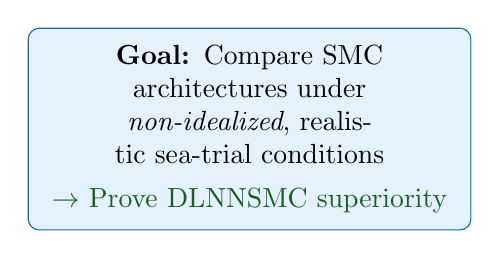
\begin{tikzpicture}
    \node[draw=midblue,fill=surfaceblue,rounded corners=4pt,
          inner sep=6pt,align=center,text width=5.2cm]{
      \textbf{Goal:} Compare SMC architectures under\\
      \emph{non-idealized}, realistic sea-trial conditions\\[4pt]
      \textcolor{okgreen}{\(\rightarrow\) Prove DLNNSMC superiority}
    };
  \end{tikzpicture}
\end{column}
\end{columns}
\end{frame}

% ══════════════════════════════════════════════════════════════════════════════
% SLIDE 3 – Problem Statement & Scope
% ══════════════════════════════════════════════════════════════════════════════
\begin{frame}{Problem Statement \& Project Scope}

\begin{columns}[T]
\begin{column}{0.48\textwidth}
  \begin{block}{Assignment Requirements}
    \begin{itemize}
      \item Reproduce \& extend a research paper
      \item Domain: \highlight{AUV} (one of 3 AUV groups)
      \item Develop hydrodynamic mathematical model
      \item Implement \& compare multiple controllers
      \item Evaluate: trajectory accuracy, stability, robustness
    \end{itemize}
  \end{block}
  \vspace{6pt}
\end{column}
\begin{column}{0.48\textwidth}
  \begin{exampleblock}{Our Contributions}
    \begin{enumerate}
      \item[\textcolor{cyancol}{\textbf{1.}}]
        \textbf{4-DOF AUV model} (extended from paper's 3-DOF)
      \item[\textcolor{cyancol}{\textbf{2.}}]
        Implemented \textbf{3 controllers} from scratch in Python
      \item[\textcolor{cyancol}{\textbf{4.}}]
        Full \textbf{Lyapunov stability proofs} documented
      \item[\textcolor{cyancol}{\textbf{5.}}]
        \textbf{2 tracking experiments}: Helix + Sinusoidal
    \end{enumerate}
  \end{exampleblock}
  \end{column}
\end{columns}
  \vspace{6pt}
  \begin{block}{Reference Paper}
  \centering
    \small
    ``Double-Loop PID-Type Neural Network Sliding Mode Control
    of an Uncertain AUV Model'',
    \textit{Mathematics}, vol.~10, no.~18, p.~3332, 2022
  \end{block}
  % \begin{tikzpicture}
  %   \node[fill=midblue,rounded corners=3pt,inner sep=5pt,text=white,
  %         text width=5.5cm,align=center]{
  %     300-second simulation \;|\; dt = 0.05 s\\
  %     Euler integration \;|\; Python
  %   };
  % \end{tikzpicture}

\end{frame}

% ══════════════════════════════════════════════════════════════════════════════
% SLIDE 4 – AUV Mathematical Model
% ══════════════════════════════════════════════════════════════════════════════
\begin{frame}{AUV Mathematical Model: 4-DOF Kinematics \& Dynamics}

\begin{columns}[T]
\begin{column}{0.46\textwidth}
  \begin{block}{State Vectors}
    \textbf{Earth-fixed} (NED frame):
    \[
      \bm{\eta} = [x,\, y,\, z,\, \psi]^\top \in \mathbb{R}^4
    \]
    \textbf{Body-fixed} velocities:
    \[
      \mathbf{v} = [u,\, v_s,\, w,\, r]^\top \in \mathbb{R}^4
    \]
    \textbf{Kinematic transform} ($\phi{=}\theta{=}0$):
    \[
      \dot{\bm{\eta}} = \mathbf{J}(\psi)\,\mathbf{v}
    \]
    \[
      \mathbf{J}(\psi)=\begin{bmatrix}c\psi & -s\psi & 0 & 0\\ s\psi & c\psi & 0 & 0\\ 0 & 0 & 1 & 0\\ 0 & 0 & 0 & 1\end{bmatrix}
    \]
  \end{block}
\end{column}
\begin{column}{0.51\textwidth}
  \begin{block}{Newton-Euler Dynamics}
    \[
      \mathbf{M}\dot{\mathbf{v}}
      + \mathbf{C}(\mathbf{v})\mathbf{v}
      + \mathbf{D}(\mathbf{v})\mathbf{v}
      + \mathbf{g}(\bm{\eta})
      = \bm{\tau} + \bm{\tau}_\text{dist}
    \]
    \vspace{-4pt}
    \begin{itemize}\small
      \item $\mathbf{M}$: inertia + added mass
            $= \text{diag}(m{-}X_{\dot{u}},\, m{-}Y_{\dot{v}},\, m{-}Z_{\dot{w}},\, I_z{-}N_{\dot{r}})$
      \item $\mathbf{C}(\mathbf{v})$: Coriolis \& centripetal
      \item $\mathbf{D}(\mathbf{v}) = \mathbf{D}_L + \mathbf{D}_Q|\mathbf{v}|$: linear + quad.\ damping
      \item $\bm{\tau}_\text{dist}$: unknown ocean current disturbances
    \end{itemize}
  \end{block}
  \vspace{4pt}
  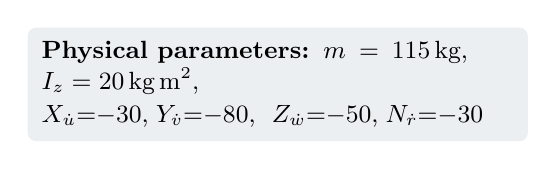
\begin{tikzpicture}
    \node[fill=tablegray,rounded corners=3pt,inner sep=5pt,
          text width=6cm,align=left]{\small
      \textbf{Physical parameters:}
      $m=115\,\text{kg}$, $I_z=20\,\text{kg\,m}^2$,\\
      $X_{\dot{u}}{=}{-30}$,\;$Y_{\dot{v}}{=}{-80}$,\;
      $Z_{\dot{w}}{=}{-50}$,\;$N_{\dot{r}}{=}{-30}$
    };
  \end{tikzpicture}
\end{column}
\end{columns}
\end{frame}

% ══════════════════════════════════════════════════════════════════════════════
% SLIDE 5 – SMC + RBFNN Foundations
% ══════════════════════════════════════════════════════════════════════════════
\begin{frame}{Control Foundations: SMC \& Radial Basis Function NNs}

\begin{columns}[T]
\begin{column}{0.47\textwidth}
  \begin{block}{Sliding Mode Control (SMC)}
    \begin{enumerate}\small
      \item Design sliding surface $\mathbf{s}$ so that $\mathbf{s}\to\mathbf{0}\Rightarrow \mathbf{e}\to\mathbf{0}$
      \item Force trajectory onto $\mathbf{s}=\mathbf{0}$ using a switching law
    \end{enumerate}
    \vspace{4pt}
    \textbf{Classic flaw — chattering:}\\
    $\bm{\tau} \propto K\,\text{sgn}(\mathbf{s})$ $\to$ infinite-frequency switching
    \[
      \boxed{\text{Fix: replace sgn with }\tanh(\mathbf{s}/\phi)}
    \]
    Continuous boundary layer eliminates actuator wear
  \end{block}
\end{column}
\begin{column}{0.50\textwidth}
  \begin{block}{Radial Basis Function Neural Network}
    Lumped unknown function $\mathbf{f}(\mathbf{v}) = \mathbf{C}\mathbf{v}+\mathbf{D}\mathbf{v}-\bm{\tau}_\text{dist}$\\[4pt]
    RBFNN approximation (Universal Approx.\ Theorem):
    \[
      \mathbf{f}(\mathbf{v}) = \mathbf{W}^{*\top}\mathbf{h}(\mathbf{v}) + \bm{\epsilon}
    \]
    Gaussian basis functions:
    \[
      h_j(\mathbf{v}) = \exp\!\left(-\frac{\|\mathbf{v}-\mathbf{c}_j\|^2}{2b_j^2}\right)
    \]
    \begin{itemize}\small
      \item Weights $\hat{\mathbf{W}}$ updated \textbf{online} — no offline training
      \item Adapts in real-time to unknown hydrodynamics \& currents
    \end{itemize}
  \end{block}
\end{column}
\end{columns}
\end{frame}

% ══════════════════════════════════════════════════════════════════════════════
% SLIDE 6 – Baseline Controllers
% ══════════════════════════════════════════════════════════════════════════════
\begin{frame}{Baseline Controllers: Single-Loop Architectures}

\begin{columns}[T]
\begin{column}{0.47\textwidth}
  \begin{block}{RBFPDSMC — PD Sliding Surface}
    Position error: $\mathbf{e} = \bm{\eta}_d - \bm{\eta}$
    \[
      \mathbf{s}_{pd} = K_p\,\mathbf{e} + K_d\,\dot{\mathbf{e}}
    \]
    Control law:
    \[
      \bm{\tau}_{pd} = \bm{\tau}_{eq} + K\tanh(\mathbf{s}_{pd}) + \hat{\mathbf{W}}^\top\mathbf{h}(\mathbf{v})
    \]
    \begin{itemize}\small
      \item Simple, fast transient response
      \item \redhl{Cannot reject constant ocean drift} (no integral)
    \end{itemize}
  \end{block}
\end{column}
\begin{column}{0.47\textwidth}
  \begin{block}{RBFPIDSMC — PID Sliding Surface}
    \[
      \mathbf{s}_{pid} = K_p\mathbf{e} + K_i\!\int\!\mathbf{e}\,dt + K_d\dot{\mathbf{e}}
    \]
    \begin{itemize}\small
      \item Integral term reduces steady-state error
      \item Still a \redhl{single-loop}: kinematics \& dynamics rigidly coupled
      \item Cannot decouple transient path planning from thrust allocation
    \end{itemize}
  \end{block}
  \vspace{6pt}
  \begin{alertblock}{Shared Limitation}
    \small Both single-loop controllers use \emph{one} sliding surface
    for both position \textbf{and} velocity — suboptimal for
    highly nonlinear, multi-DOF marine systems
  \end{alertblock}
\end{column}
\end{columns}
\end{frame}

% ══════════════════════════════════════════════════════════════════════════════
% SLIDE 7 – DLNNSMC Architecture
% ══════════════════════════════════════════════════════════════════════════════
\begin{frame}{Proposed DLNNSMC: Double-Loop Architecture}

\begin{center}
\resizebox{0.96\textwidth}{!}{%
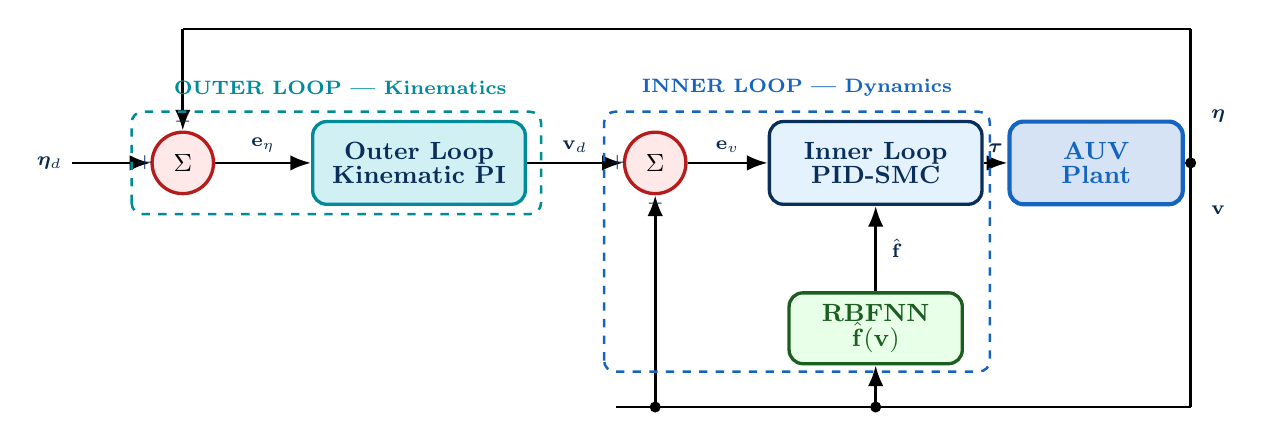
\begin{tikzpicture}[
  >=Latex,
  block/.style={draw=oceanblue,fill=surfaceblue,rounded corners=5pt,
                minimum width=2.7cm,minimum height=1.05cm,
                align=center,font=\small\bfseries,line width=1.2pt},
  nn/.style={draw=okgreen,fill=green!9,rounded corners=5pt,
             minimum width=2.2cm,minimum height=0.9cm,
             align=center,font=\small\bfseries,line width=1.2pt},
  plant/.style={draw=midblue,fill=midblue!18,rounded corners=5pt,
                minimum width=2.2cm,minimum height=1.05cm,
                align=center,font=\small\bfseries,line width=1.5pt},
  sum/.style={circle,draw=warnred,fill=red!9,minimum size=0.78cm,
              inner sep=0pt,font=\small\bfseries,line width=1.2pt},
  sig/.style={font=\scriptsize,color=oceanblue!85!black}
]

%% ── Block placement (all at explicit absolute coordinates) ──
\node[sum]   (S1)  at (0,0)     {$\Sigma$};
\node[block, fill=cyancol!18, draw=cyancol!80!black]
             (OL)  at (3.0,0)   {\textcolor{oceanblue}{Outer Loop}\\[-2pt]
                                  \textcolor{oceanblue}{Kinematic PI}};
\node[sum]   (S2)  at (6.0,0)   {$\Sigma$};
\node[block] (IL)  at (8.8,0)   {\textcolor{oceanblue}{Inner Loop}\\[-2pt]
                                  \textcolor{oceanblue}{PID-SMC}};
\node[plant] (AUV) at (11.6,0)  {\textcolor{midblue}{AUV}\\[-2pt]
                                  \textcolor{midblue}{Plant}};
\node[nn]    (NN)  at (8.8,-2.1){\textcolor{okgreen}{RBFNN}\\[-2pt]
                                  \textcolor{okgreen}{$\hat{\mathbf{f}}(\mathbf{v})$}};
\node[sig, left=1.0cm of S1] (etad) {$\bm{\eta}_d$};

%% ── Forward path ──
\draw[->, line width=1pt] (etad) -- (S1);
\draw[->, line width=1pt] (S1)  -- node[above,sig]{$\mathbf{e}_\eta$} (OL);
\draw[->, line width=1pt] (OL)  -- node[above,sig]{$\mathbf{v}_d$}   (S2);
\draw[->, line width=1pt] (S2)  -- node[above,sig]{$\mathbf{e}_v$}   (IL);
\draw[->, line width=1pt] (IL)  -- node[above,sig]{$\bm{\tau}$}      (AUV);
\draw[->, line width=1pt] (NN.north)
  -- node[right,sig,xshift=2pt]{$\hat{\mathbf{f}}$} (IL.south);

%% ── AUV output junction at (12.8, 0) ──
\draw[line width=1pt] (AUV.east) -- (12.8, 0);
\fill (12.8, 0) circle (2pt);         % junction dot

%% η branch: go UP from junction
\draw[line width=1pt] (12.8, 0) -- (12.8, 0.6);
\node[sig] at (13.15, 0.6) {$\bm{\eta}$};

%% v branch: go DOWN from junction
\draw[line width=1pt] (12.8, 0) -- (12.8,-0.6);
\node[sig] at (13.15,-0.6) {$\mathbf{v}$};

%% ── η feedback: top rail at y = 1.70 ──
%   (12.8, 0.6) → up → (12.8, 1.70) → left → (0, 1.70) → down → S1.north
\draw[line width=1pt] (12.8,  0.6) -- (12.8, 1.70);
\draw[line width=1pt] (12.8, 1.70) -- (0.0,  1.70);
\draw[->, line width=1pt] (0.0, 1.70) -- (S1.north);

%% ── v feedback: bottom rail at y = -3.10 ──
%   (12.8,-0.6) → down → (12.8,-3.10) → left → (5.5,-3.10)
%   Tap 1: (6.0,-3.10) → up → S2.south
%   Tap 2: (8.8,-3.10) → up → NN.south
\draw[line width=1pt] (12.8, -0.6) -- (12.8, -3.10);
\draw[line width=1pt] (12.8,-3.10) -- (5.5,  -3.10);

\fill (6.0,-3.10) circle (2pt);       % tap junction dot
\draw[->, line width=1pt] (6.0,-3.10) -- (S2.south);

\fill (8.8,-3.10) circle (2pt);       % tap junction dot
\draw[->, line width=1pt] (8.8,-3.10) -- (NN.south);

%% ── Summing node signs ──
% S1: etad from west (+), eta feedback from north (-)
\node[sig] at (-0.48,  0.0) {$+$};
\node[sig] at (  0.0,  0.52) {$-$};
% S2: vd from west (+), v feedback from south (-)
\node[sig] at (5.52,   0.0) {$+$};
\node[sig] at (6.0,   -0.52) {$-$};

%% ── Loop bounding boxes ──
\draw[dashed,cyancol!80!black,rounded corners=4pt,line width=0.9pt]
  (-0.65,-0.65) rectangle (4.55, 0.65);
\node[cyancol!80!black,font=\scriptsize\bfseries] at (2.0, 0.95)
  {OUTER LOOP --- Kinematics};

\draw[dashed,midblue,rounded corners=4pt,line width=0.9pt]
  (5.35,-2.65) rectangle (10.25, 0.65);
\node[midblue,font=\scriptsize\bfseries] at (7.80, 0.95)
  {INNER LOOP --- Dynamics};

\end{tikzpicture}
}
\end{center}

\vspace{-6pt}
\begin{columns}[T]
\begin{column}{0.47\textwidth}
  \begin{block}{\small Outer Loop - Virtual Velocity}
    \vspace{3pt}
    \[
      \mathbf{v}_d = \mathbf{J}^{-1}\!\left(\dot{\bm{\eta}}_d
        + K_{p,\text{out}}\mathbf{e}_\eta
        + K_{i,\text{out}}\!\textstyle\int\!\mathbf{e}_\eta\right)
    \]
  \end{block}
\end{column}
\begin{column}{0.47\textwidth}
  \begin{block}{\small Inner Loop - Thrust Torque}
    \[
      \bm{\tau} = \mathbf{M}(\dot{\mathbf{v}}_d + C_{in}\mathbf{e}_v)
      + K\tanh(\mathbf{s}) + \hat{\mathbf{W}}^\top\mathbf{h}(\mathbf{v})
    \]
  \end{block}
\end{column}
\end{columns}
\end{frame}

% ══════════════════════════════════════════════════════════════════════════════
% SLIDE 8 – Lyapunov Stability
% ══════════════════════════════════════════════════════════════════════════════
\begin{frame}{Lyapunov Stability Analysis}
\small % Slightly reduce font size for the whole frame to ensure fit

\begin{columns}[T, onlytextwidth]
  % --- Left Column ---
  \begin{column}{0.48\textwidth}
    \begin{block}{Candidate Lyapunov Function}
      \[
        V = \frac{1}{2}\mathbf{s}^\top\mathbf{M}\mathbf{s} 
        + \frac{1}{2}\operatorname{tr}\!\left(\tilde{\mathbf{W}}^\top \Gamma^{-1}\tilde{\mathbf{W}}\right)
      \]
      \scriptsize where $\tilde{\mathbf{W}} = \hat{\mathbf{W}} - \mathbf{W}^*$ is weight error, $\Gamma > 0$ is adaptation gain.
    \end{block}

    \begin{block}{Weight Adaptation Law}
      Derived to cancel error terms:
      \[
        \dot{\hat{\mathbf{W}}} = \Gamma\,\mathbf{h}(\mathbf{v})\,\mathbf{s}^\top
      \]
    \end{block}
  \end{column}

  \hfill

  % --- Right Column ---
  \begin{column}{0.48\textwidth}
    \begin{block}{Stability Proof (Key Steps)}
      \textbf{Step 1} — Time derivative:
      \[
        \dot{V} = \mathbf{s}^\top\mathbf{M}\dot{\mathbf{s}} 
        + \operatorname{tr}\!\left(\tilde{\mathbf{W}}^\top\Gamma^{-1}\dot{\hat{\mathbf{W}}}\right)
      \]
      \textbf{Step 2} — Substitute control law:
      \[
        \dot{V} = -\mathbf{s}^\top K\tanh(\mathbf{s}) + \mathbf{s}^\top\bm{\epsilon}
      \]
      \textbf{Step 3} — Bound:
      \[
        \dot{V} \leq -K_{\min}\|\mathbf{s}\| + \epsilon_{\max}\|\mathbf{s}\|
      \]
    \end{block}
  \end{column}
\end{columns}

\vspace{4pt}

% --- Bottom Guarantee (Full Width to save vertical space) ---
\begin{exampleblock}{Guarantee}
  If $K_{\min} > \epsilon_{\max} \implies \dot{V} < 0$. 
  By \textbf{Barbalat's Lemma}: $\mathbf{s}\to\mathbf{0}$, hence $\mathbf{v}\to\mathbf{v}_d$ and $\bm{\eta}\to\bm{\eta}_d$ asymptotically.
\end{exampleblock}

\end{frame}
% ══════════════════════════════════════════════════════════════════════════════
% SLIDE 9 – Simulation Setup
% ══════════════════════════════════════════════════════════════════════════════
\begin{frame}{Simulation Setup \& Realism Constraints}

\small % Global small font for dense content

\begin{columns}[T, onlytextwidth]

% --- Left Column: Realism Constraints ---
\begin{column}{0.49\textwidth}

\begin{alertblock}{4 Injected Realism Constraints}

\begin{enumerate}[leftmargin=1.2em]

\item \textbf{15\% model mismatch:}\\
$\hat{\mathbf{M}} = 0.85 \times \mathbf{M}_\text{true}$

\item \textbf{Acoustic sensor noise:}\\
{\scriptsize
$\eta_\text{meas}
=
\eta_\text{true}
+
\mathcal{N}(0, 0.02^2)$\\
$v_\text{meas}
=
v_\text{true}
+
\mathcal{N}(0, 0.01^2)$}

\item \textbf{Harmonic ocean currents:}\\
{\scriptsize
$\tau_\text{dist}
=
8\sin(0.05t)
+
3\cos(0.02t)
+
\mathcal{N}(0,1)$}\\
\textit{\scriptsize (Up to 8\,N sustained drift)}

\item \textbf{Actuator saturation:}\\
$\tau \in [-800,\,+800]$\,N limit

\end{enumerate}

\end{alertblock}

\end{column}

\hfill

% --- Right Column ---
\begin{column}{0.48\textwidth}

% --- Simulation Parameters Table ---
\begin{block}{Simulation Parameters}

\centering
\scriptsize

\begin{tabular}{lc}
\toprule
Parameter & Value \\
\midrule
Duration & 300 s \\
Timestep $dt$ & 0.05 s \\
Integration & Euler \\
Vehicle mass $m$ & 115 kg \\
Yaw inertia $I_z$ & 20 kg\,m$^2$ \\
RBFNN nodes & 7 per DOF \\
Boundary layer $\phi$ & 0.1 \\
\bottomrule
\end{tabular}

\end{block}

\vspace{3pt}

% --- Green Box (Fixed Alignment) ---
\begin{exampleblock}{Two Tracking Scenarios}

\textbf{Exp 1:} 3-D Ascending Helix\\
{\scriptsize Tests transient \& sustained tracking}

\vspace{4pt}

\textbf{Exp 2:} 3-D Spatial Sinusoidal\\
{\scriptsize Tests yaw/sway coupling}

\end{exampleblock}

\end{column}

\end{columns}

\end{frame}

% ══════════════════════════════════════════════════════════════════════════════
% SLIDE 10 – Exp 1: Helix Trajectory (plot + GIF placeholder)
% ══════════════════════════════════════════════════════════════════════════════
\begin{frame}{Experiment 1: Ascending Helix — 3D Trajectory}

\begin{columns}[T, onlytextwidth]

% --- Left Column: Static Trajectory ---
\begin{column}{0.55\textwidth}

\centering


\includegraphics[
    width=\textwidth,
    height=0.65\textheight,
    keepaspectratio
]{exp1_3d_trajectory.png}

\end{column}

\hfill

% --- Right Column: Animation + Notes ---
\begin{column}{0.40\textwidth}

% --- GIF Placeholder (Fixed Scaling) ---
\centering

% \begin{tikzpicture}[scale=0.75]

% \fill[tablegray,rounded corners=4pt]
% (0,0) rectangle (5.0,3.6);

% \draw[midblue,dashed,rounded corners=4pt,line width=1pt]
% (0.15,0.15) rectangle (4.85,3.45);

% \fill[midblue]
% (2.2,2.2) -- (2.8,2.6) -- (2.2,3.0) -- cycle;

% \node[midblue,font=\small\bfseries]
% at (2.5,1.8)
% {Animation};

% \node[midblue!70,font=\footnotesize,align=center]
% at (2.5,1.2)
% {exp1\_combined\_trajectory.gif};

% \node[midblue!50,font=\scriptsize,align=center]
% at (2.5,0.6)
% {(Insert GIF in final slides)};

% \end{tikzpicture}

\vspace{6pt}

% --- Observations ---
\begin{block}{\small Key Observations}

\footnotesize

\begin{itemize}

\item Orange dot = AUV start (offset from path)

\item \textcolor{warnred}{\textbf{Red (RBFPD)}}:
noisy, wide deviation

\item \textcolor{okgreen}{\textbf{Green (RBFPID)}}:
smoother but still overshoots

\item \textcolor{dlnncolor}{\textbf{Blue (DLNN)}}:
locks onto path within
\textbf{$\sim$25 s}

\item DLNN tracks the figure-8 base tightly

\end{itemize}

\end{block}

\end{column}

\end{columns}

\end{frame}
% ══════════════════════════════════════════════════════════════════════════════
% SLIDE 11 – Exp 1: Error Analysis
% ══════════════════════════════════════════════════════════════════════════════
\begin{frame}{Experiment 1: Position Tracking Errors}

\begin{columns}[T, onlytextwidth]

% --- Left Column: Image and Aligned Labels ---
\begin{column}{0.60\textwidth}
  \centering

  
\includegraphics[
      width=\textwidth,
      height=0.65\textheight,
      keepaspectratio
  ]{exp1_position_errors.png}

  \vspace{2pt}

  % Aligned subplot labels
  \begin{tabular}{p{0.45\textwidth} p{0.45\textwidth}}
    \centering\scriptsize (a) $x_e$ [m], (b) $y_e$ [m] &
    \centering\scriptsize (c) $z_e$ [m], (d) $\psi_e$ [rad]
  \end{tabular}

\end{column}

\hfill

% --- Right Column: Analysis Blocks ---
\begin{column}{0.37\textwidth}

  \begin{block}{\small Error Analysis}
    \footnotesize
    \begin{itemize}
      \item \textbf{$x_e$, $z_e$:}
      DLNN stays within tight $\pm0.05$ m band.

      \item \textbf{$y_e$:}
      Baselines show undulating error —
      unable to reject slow harmonic current.

      \item \textbf{$\psi_e$:}
      DLNN converges to $\approx 0$ rad,
      baselines oscillate at $\mathbf{0.25}$ rad.
    \end{itemize}
  \end{block}

  \vspace{1.5pt}

  \begin{alertblock}{\small Why Baselines Fail}
    \footnotesize
    Single sliding surface cannot simultaneously compensate
    for both the kinematic path error \emph{and}
    the current-induced torque mismatch.
  \end{alertblock}

  \vspace{1.5pt}

  \begin{exampleblock}{\small DLNN Advantage}
    \footnotesize
    RBFNN maps harmonic drift frequencies online,
    rendering the controller dynamically invariant to them.
  \end{exampleblock}

\end{column}

\end{columns}

\end{frame}

% ══════════════════════════════════════════════════════════════════════════════
% SLIDE 12 – Exp 2: Sinusoidal Trajectory
% ══════════════════════════════════════════════════════════════════════════════
\begin{frame}{Experiment 2: Spatial Sinusoidal — 3D Trajectory}

\begin{columns}[T, onlytextwidth]
  % --- Left Column: 3D Static Plot ---
  \begin{column}{0.54\textwidth}
    \centering
    
\includegraphics[width=\textwidth, height=0.7\textheight, keepaspectratio]{exp2_3d_trajectory.png}\\[4pt]
    {\scriptsize 3D Position tracking performance}
  \end{column}

  \hfill

  % --- Right Column: Animation & Notes ---
  \begin{column}{0.43\textwidth}
    \centering
    % Direct GIF loading (Note: Requires a compiler/viewer that supports GIFs, like LuaLaTeX/HTML outputs, otherwise use a PNG frame here)
    \includegraphics[width=0.9\textwidth, height=4cm, keepaspectratio]{exp2_combined_trajectory.gif}

    \vspace{10pt}

    \begin{block}{\small Key Observations}
      \scriptsize
      \begin{itemize}
        \setlength{\itemsep}{2pt}
        \item Sinusoidal path demands repeated sharp yaw reversals.
        \item \textcolor{red}{\textbf{Red}}/\textcolor{green}{\textbf{Green}}: consistently \textbf{undershoot} the apex (``cut corners'').
        \item \textcolor{blue}{\textbf{Blue (DLNN)}}: Traces outer boundary with high precision.
        \item Decoupled inner loop handles high-freq dynamics effectively.
      \end{itemize}
    \end{block}
  \end{column}
\end{columns}

\end{frame}
% ══════════════════════════════════════════════════════════════════════════════
% SLIDE 13 – Exp 2: Error Analysis
% ══════════════════════════════════════════════════════════════════════════════
\begin{frame}{Experiment 2: Position Tracking Errors}

\begin{columns}[T, onlytextwidth]
  % --- Left Column: Image and Aligned Labels ---
  \begin{column}{0.60\textwidth}
    \centering
    
\includegraphics[width=\textwidth, height=0.65\textheight, keepaspectratio]{exp2_position_errors.png}
    
    \vspace{2pt}
    % This table keeps labels perfectly aligned with the plots above
    \begin{tabular}{p{0.45\textwidth} p{0.45\textwidth}}
      \centering\scriptsize (a) $x_e$ [m], (b) $y_e$ [m] & 
      \centering\scriptsize (c) $z_e$ [m], (d) $\psi_e$ [rad]
    \end{tabular}
  \end{column}

  \hfill

  % --- Right Column: Analysis Blocks ---
  \begin{column}{0.37\textwidth}
    \begin{block}{\small Observations: $\psi_e$}
      \footnotesize
      \begin{itemize}
        \item \textbf{Baselines:} $\psi_e$ oscillates at $\pm 0.20$ rad persistently.
        \item \textbf{DLNN:} Error converges to $\approx 0$ within 30s.
        \item Handles high-frequency heading switching.
      \end{itemize}
    \end{block}

    \begin{alertblock}{\small $z_e$ Comparison}
      \footnotesize
      \textbf{Baselines:} Drift $\pm 0.10$ m.\\
      \textbf{DLNN:} Bounded $\pm 0.03$ m.\\
      \textit{Ideal for pipeline inspection.}
    \end{alertblock}
  \end{column}
\end{columns}

\end{frame}
% ══════════════════════════════════════════════════════════════════════════════
% SLIDE 14 – RMSE Results
% ══════════════════════════════════════════════════════════════════════════════
\begin{frame}{Quantitative Results: RMSE Comparison}

\begin{center}
\begin{tabular}{lcccccc}
  \toprule
  & \multicolumn{3}{c}{\textbf{Experiment 1: Ascending Helix}}
  & \multicolumn{3}{c}{\textbf{Experiment 2: Sinusoidal}} \\
  \cmidrule(lr){2-4}\cmidrule(lr){5-7}
  \textbf{Controller}
    & $x_e$ [m] & $y_e$ [m] & $z_e$ [m]
    & $x_e$ [m] & $y_e$ [m] & $z_e$ [m] \\
  \midrule
  \rowcolor{red!12}
  RBFPDSMC
    & 0.0481 & 0.0539 & 0.0417
    & 0.0575 & 0.0390 & 0.0413 \\
  \rowcolor{yellow!15}
  RBFPIDSMC
    & 0.0414 & 0.0391 & 0.0356
    & 0.0471 & 0.0347 & 0.0346 \\
  \rowcolor{green!15}
  \textbf{DLNNSMC (Ours)}
    & \textbf{0.0261} & \textbf{0.0228} & \textbf{0.0258}
    & \textbf{0.0257} & \textbf{0.0258} & \textbf{0.0261} \\
  \bottomrule
\end{tabular}
\end{center}

\vspace{10pt}
\begin{columns}[T]
\begin{column}{0.30\textwidth}
  \begin{exampleblock}{\centering vs.\ RBFPDSMC}
    \centering
    {\Large\bfseries\color{okgreen}$\downarrow$45.7\%}\\
    {\small to 50.1\% RMSE reduction}
  \end{exampleblock}
\end{column}
\begin{column}{0.30\textwidth}
  \begin{exampleblock}{\centering vs.\ RBFPIDSMC}
    \centering
    {\Large\bfseries\color{okgreen}$\downarrow$30.2\%}\\
    {\small to 38.5\% RMSE reduction}
  \end{exampleblock}
\end{column}
\begin{column}{0.36\textwidth}
  \begin{block}{Why DLNNSMC Wins}
    \begin{itemize}\small
      \item Kinematic \& dynamic loops independently optimized
      \item RBFNN absorbs all unmodeled disturbances
      \item $\tanh$ smoothing eliminates chattering
    \end{itemize}
  \end{block}
\end{column}
\end{columns}
\end{frame}

% ══════════════════════════════════════════════════════════════════════════════
% SLIDE 15 – Conclusion & Future Work
% ══════════════════════════════════════════════════════════════════════════════
\begin{frame}{Conclusion \& Future Directions}
\small 

\begin{columns}[T, onlytextwidth]
  % --- Left Column: Summary ---
  \begin{column}{0.49\textwidth}
    \begin{exampleblock}{Summary of Findings}
      \begin{itemize}
        \item Successfully replicated paper
        \item Built 4-DOF AUV Python simulation
        \item \textbf{DLNNSMC achieves 50\% lower RMSE}
        \item Lyapunov proof confirms stability
        \item $\tanh$ layer ensures \textbf{no chattering}
        \item Robust to 15\% mismatch \& noise
      \end{itemize}
    \end{exampleblock}
  \end{column}

  \hfill

  % --- Right Column: Future & Highlight ---
  \begin{column}{0.48\textwidth}
    \begin{block}{Future Directions}
      \footnotesize
      \begin{enumerate}
        \item[\textbf{1.}] \textbf{HIL Testing}: Deploy in C++/ROS on Nvidia Jetson Nano.
        \item[\textbf{2.}] \textbf{6-DOF}: Add pitch/roll for complex maneuvers.
        \item[\textbf{3.}] \textbf{Vision}: Use visual odometry for current estimation.
      \end{enumerate}
    \end{block}
  \end{column}
\end{columns}

\vfill

% --- Fixed Footer ---
% \begin{center}
%   {\color{gray}\rule{8cm}{0.4pt}}\\[3pt]
%   {\scriptsize \textbf{Marine Robotics Course Project} --- Nitesh \textbullet\ Dhruv \textbullet\ Suchit \textbullet\ Surya}
% \end{center}

\end{frame}
\end{document}
